\chapter{Original methodology for a computer aided forensic audit}
\komentar{Jsem si vedoma, ze jsem clovek, ktery to nikdy nedelal (= omezena znalost).
Toto je jak to chapu. Toto neni jak by to nekdo mel delat. Toto je seriozni pokus popsat proces forenzniho auditu.
PROCESNI DIAGRAMY!!!

vystupem = okomentovany obrazek, ktery dava hlavu a patu

s Use case diagrammem pak kontaktovat praxi

}


We are aware to have only limited knowledge of forensic audit and no practical experience. This chapter should not be considered as a manual explaining how forensic audit should be done.  However, this is rather a serious attempt to describe the process of forensic audit.


%=====================================================================================
\section{The phase of preparation of the forensic-audit process}
Before the process of forensic audit starts there is a block of organizational or administrative affairs that needs to be \anglictina{done}. It all starts in a institution where there is a suspicion of an act that is not following required rules. The institution might be of various kinds. A example can be an international corporation suspecting one of local branches from a money leakage. \komentar{dalsi priklady?}

The rules might be either internal regulation or corporate policies or even given by law. Basically any kind of misbehavior can be investigated by forensic audit. Given the background of the case the ordering party might also be of multiple kinds and from various branches of economy. They usually suspect possible internal or external risks that can be represented by fraudsters or people committing some other type of crime.  Generally the ordering party is the head of a given company. Some specific cases are: CEO of certain company, new holder of an existing company, authorized representative of a supervisory board etc.. However forensic audit can be also assigned by a court or the police. 

After the decision to perform forensic audit the ordering party contacts the audit company and they negotiate with a business representative about the sphere of the contract, price and deadlines. If there is no agreement it is probable that the ordering party contacts another audit company. It is important to familiarize the ordering party with the fact that while conducting forensic audit the auditors might need access to various confidential information concerning the ordering company. On the other hand the audit company undertakes not not to manipulate with this data in a protective way and not to expose it to the risk of misuse. If both parties agree with the conditions the contract is made and the case is accepted. 

In the audit company there is a team of specialists established according to the character of the case. It is important to be aware of conflict of interest in this phase. Members of the team must not be related in any way to the original case. Members of the team can be forensic auditors, data analytics, specialists in any particular field (biometry, data recovery, criminology, law, etc.), consultants and assistants. 

When the team of auditors is established the next thing is creating a document for record of the investigation. It also serves as a documentation. It is also common to create a nickname for important subjects and for the case to provide security of the confidential information. This is the end of all the administration that needs to be done before the actual forensic audit. 

%=====================================================================================
\section{Accumulation of data}
In the beginning of the investigation the team needs to gain an insight into the background situation of the case. They can learn it from materials they have been provided by the client. An appropriate strategy for investigation is created. It means, that all the relevant methods are taken account of and the best are chosen. 

In all the cases it is important to secure all the documents, data repositories and all other possible sources of (digital) evidence. Any unauthorized person must not have a chance to manipulate with any possible evidence. For this reason backups of all the digital information are made. According to a FBI statistics the average investigated case size is approximately 500 GB. \komentar{citace (ariu- paper, zdroj 13)} In fact there are usually two copies of the data. The first is utterly for backup and the second can be used for analysis and work with the data. 

The investigating team needs to evaluate all possible available sources of important information, access and gain the data. If the case is somehow special it might be needed to authorize an specialist to collect specific pieces of evidence. An example could be a case when fingerprint recording is needed. 

It might be useful to visit the workplace of the investigated company and check if there are some other possible sources of evidence. After having all the data secured in some cases it can be also beneficial to perform a cross examination. It can be done even by mere conversation with involved persons, but it should be recorded.

It is possible that already in the end of collection of data the forensic audit team has a idea or even hypothesis about what happened in the chase. Having this idea might be useful in further investigation, but auditors should beware of jumping into conclusions. All the actions and also the potential hypothesis should be documented in the case documentation. 

%=====================================================================================
\section{Examination}

The phase of examination comes when all the data is collected. Methods of examination are very different according to the character of the case, the sources of data and also the field that is investigated. 

In the examination phase it is necessary at first to assess the data and mine the relevant pieces of information from all the collected data. It starts by identification of the data files that contain information of interest. Forensic auditors must not be discouraged by the size of data. After those files are identified it is often demanded to filter the extraneous information and leave only the coarsely filtered data. 

%=====================================================================================
\section{Analysis}
After the data being pre-filtered there comes the most extensive part of the investigation. The aim of analysis is to study and analyze the data to draw conclusions from it or to determine that no conclusion can be drawn. By the end of analysis most important subjects, events, people, and people and relationships between them should be recognized. In order to find the conclusion it is required to unite information gained from multiple sources of data.

However first of all to obtain the information hidden in the data, specific sources of data need to be analyzed by a competent specialist. For example provided that a file contains billing data the task is delegated to accountancy specialists. They can use appropriate accounting software, or extract only data of particular interest and use some quantitative software. If the data contain log files, or deleted files it is a job for information technology specialists to recover or examine the data. 


Several methods the team of investigators might use are: quantitative software analysis, analysis of relationships between persons, making use of analytical software. In case of  suspicion from corruption a investigation of decisions made by the management of the company might be needed. Investigators might pose questions similar to following. Who are the suppliers of the investigated company? In what business the company invests and who decides about it? Who does have an access to (financial) resources?


There might be cases when specialists in various sub-branches of forensics might be needed. Even an external company might be hired to solve a particular problem. Examples of auxiliary specialists can be experts in computer forensics, forensic dactylography, digital forensics, forensic biometry, forensic psychiatry, forensic linguistic etc. According to all available expert's opinions the situation in the case is gradually revealed.

All the steps proceeded in the analysis result in understanding of the situation in the case. According to the information investigators gained a verdict is pronounced and retrospectively supported by the data collected in the beginning of the process. 

%=====================================================================================
\section{Reporting}

After having investigated the assigned case the team of forensic auditors has some results to show. Either they have found what undesirable actions happened or there might be cases when they have not discovered any signs of such behavior. In both cases proper results are presented to the ordering party. 


If a crime has been discovered and evidence denoting the the actions leading to the crime has been revealed the situation as it happened must be properly described and explained in the presentation to the ordering party. 

\komentar{
- posledni faze\\
- priprava na prezentaci vysledku\\
- vytvoreni alternativnich reseni (pokud mame nekompletni informace o tom, co se stalo)\\
- zvazeni komu budou vysledky prezentovane\\
- navrhy opatreni vzhledem k vysledkum forenzniho auditu\\
- oznameni jinych problemu na ktere se mimochodem pri vysetrovani prislo\\
- navrhy ve vylepseni procesu a smernic (ve firme)\\


DALE:\\
- rozsireni expertizy auditorske spolecnosti, ale s ohledem na citlivos dat v danem pripadu
- sledovani trendu v technologiich a novelach zakonu

}



\colorbox{green}{\komentar{ timhle diagramem bude problem, budu ho muset prinutit aby se rozdelil na vic stran}}

\begin{figure}[h]
	\begin{center} 
	%\missingfigure{Velky obrazek vsech zainteresovanych stran - f.auditor, datovy analytik pro FA, zakaznik (zadavatel, materska spolecnost)}
	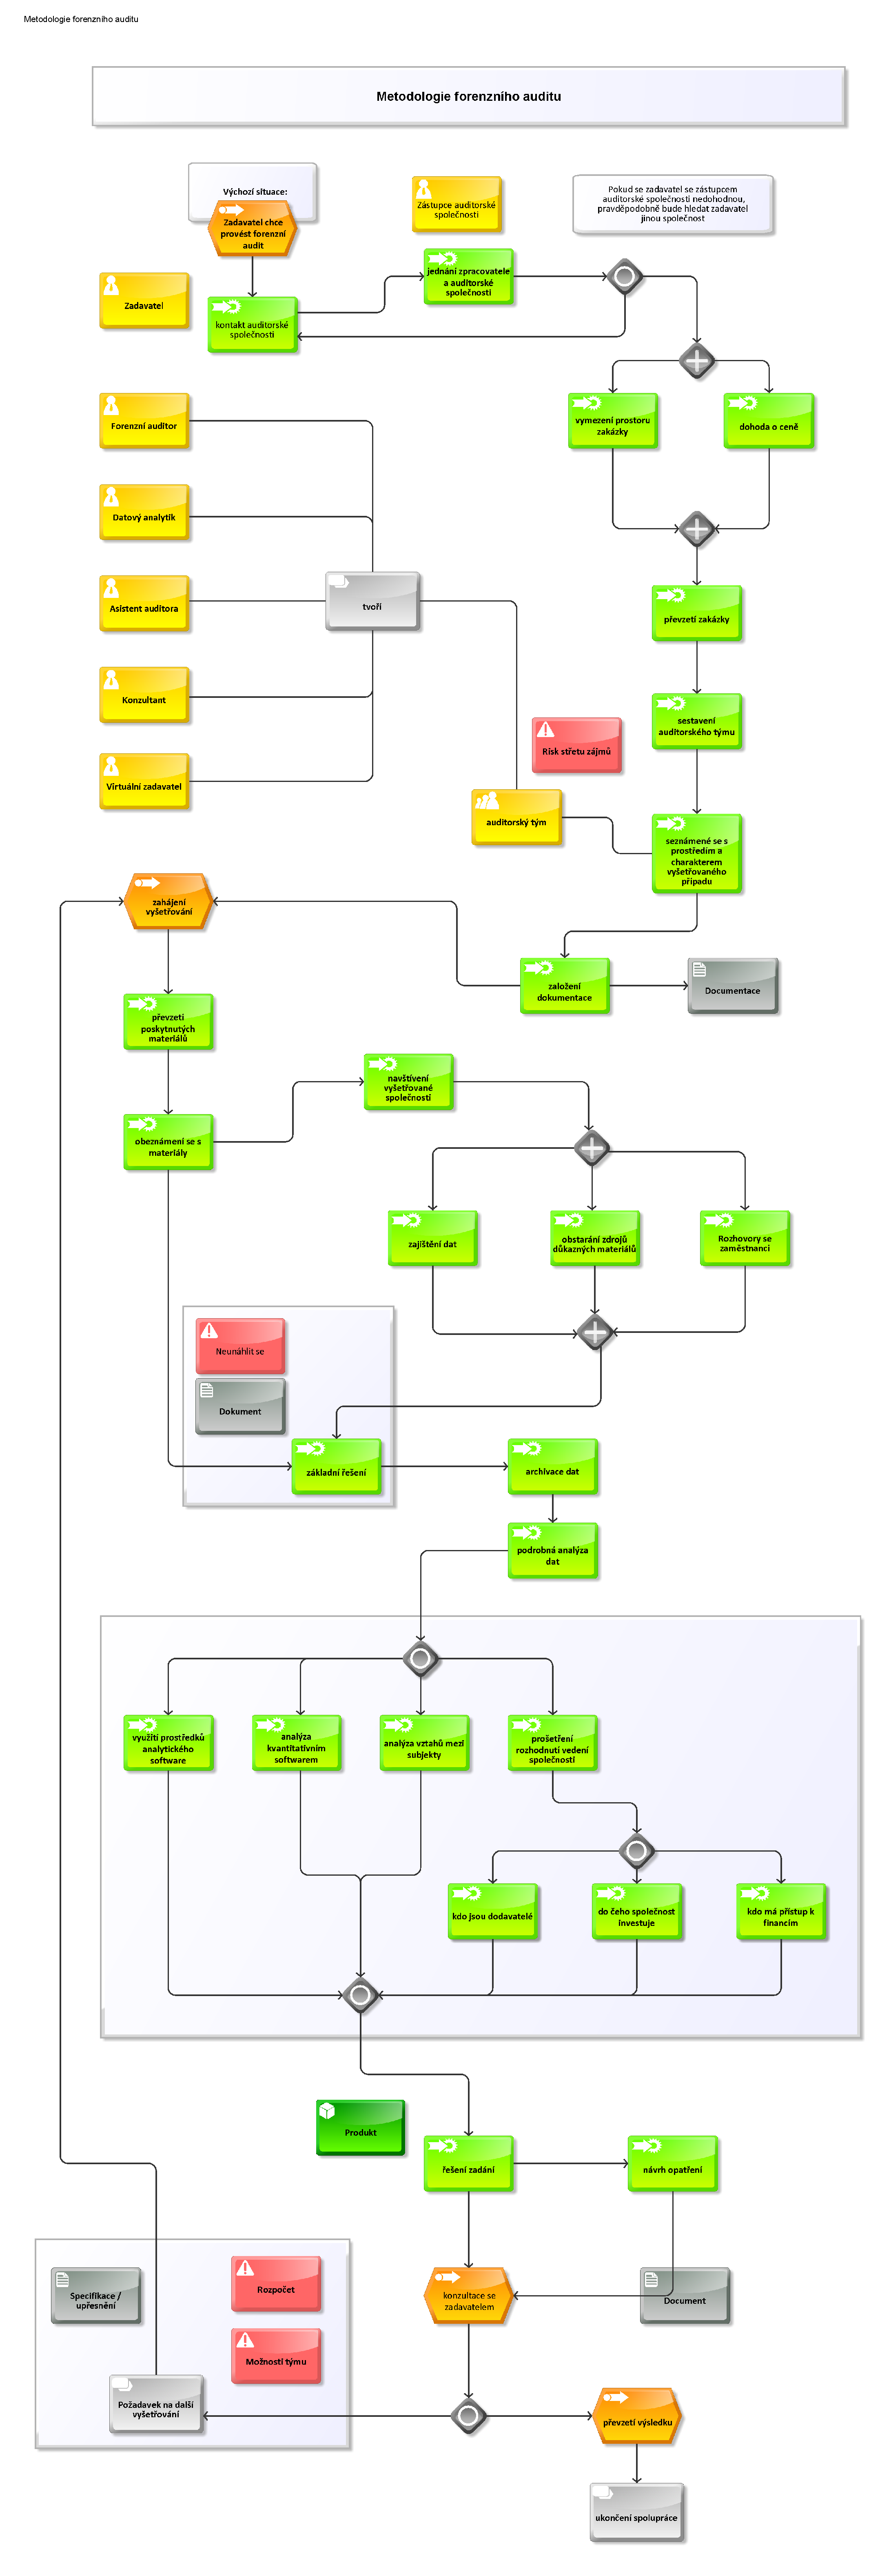
\includegraphics[width=1.0\textwidth]{img/metodika/Metodologie_forenzniho_auditu.pdf}
	\end{center}
	\caption{\komentar{Metodika v ARISu}}
\end{figure}

 
